\documentclass[10pt,notitlepage]{article}
\usepackage{graphicx}
\usepackage{verbatim}
\usepackage[portuguese]{babel}
\usepackage[utf8]{inputenc}
\usepackage[hmargin=2cm,vmargin=3.5cm,bmargin=2cm]{geometry}


\begin{document}

%%%CAPA%%%

\begin{figure}
\centering

\includegraphics[scale=0.5]{logo.pdf}
\end{figure}

$\\$
$\\$

\begin{center}

Escola de Engenharia \\~ \\~ \\~  Departamento de Informática \\~ \\ ~ \\~ Licenciatura em Engenharia Informática \\~ \\~ \\~ Programação Orientada aos Objectos \\~ \\~ \\~ \\~ \\~ \\~ \\~  Projecto Java - FitnesUM \\~ \\~ \\~ \\~ \\~ \\~ \\~
\begin{figure}[h]
\centering
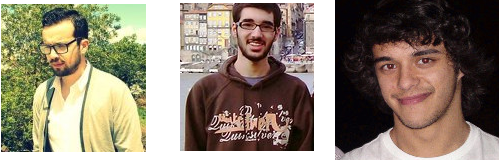
\includegraphics[scale=0.6]{autores.png}
\caption{Autores (a),(b),(c)}
\end{figure}

A69854 ~~~~~~~~~~~~~~~~~~ A66822 ~~~~~~~~~~~~~~~~~~ A   \\~  João Mano ~~~~~~~~ Miguel Guimarães ~~~~~~~~ Bruno Torres  \\~ \\~ \\~ \\~ \\~ \\~ Braga, Junho de 2014
\end{center}

\newpage


\tableofcontents

\newpage


\section{Estrutura da aplicação}

\subsection{Classe abstracta Activity}

Esta é a classe mais abstrata, que tem a fundação de todas as actividadades desta aplicação. Contém variáveis comuns a todas as actividades, \textit{name}, \textit{date}, \textit{timeSpent} e \textit{calories} tal como os construtores, \textit{getters} e  \textit{setters}.

\begin{figure}[h]
\centering
\includegraphics[scale=0.6]{actividades.jpeg}
\end{figure}



\end{document}

















